\documentclass[hyperref={pdfpagemode=FullScreen, colorlinks=false}]{beamer}

\usepackage{selinput}			% Inputencoding
	\SelectInputMappings{adieresis={ä}, germandbls={ß}, Euro={€}}
\usepackage[T1]{fontenc}		% Fontencoding
%
\usepackage{pifont}
\usepackage{csquotes,siunitx}			% Anführungszeichen; wird von biblatex gewünscht
\usepackage[backend=biber,citestyle=alphabetic,uniquelist=false]{biblatex}	% Literatur formatieren
\addbibresource{bodendynamik.bib}	% Literaturdatenbank
\usepackage{caption} 
\usepackage{subfig}
\usepackage{comment}
%%%%%%%%%%%%%%%%%%%%%%%%%%%%%%%%%%%%%%%%%%%%%%%%%%%%%%%%%%%%%%%%%%%%%%%%%%%%%%%%%%%%%%%%%%%%%%%%%%%%%%%
% Thema für Präsentation
\usetheme[fusszeile=ernstcolor,sprache=ngerman,seite=letzte,
verhaeltnis=16:10,
hausschrift=false,
navigation=false,
titelseite=blau]{TUBAF}

\TUBAFZweitlogo{
\includegraphics{fig_pdf/UFZ_logo_inv.pdf}}

%%%%%%%%%%%%%%%%%%%%%%%%%%%%%%%%%%%%%%%%%%%%%%%%%%%%%%%%%%%%%%%%%%%%%%%%%%%%%%%%%%%%%%%%%%%%%%%%%%%%%%%
% Optionen für Anmerkungen
\mode<presentation>{%
\setbeameroption{hide notes}				% keine Notizen (default)
%\setbeameroption{show notes}				% Notizen und Frames gemischt
%\setbeameroption{show only notes}			% nur Notizen
%
%\usepackage{pgfpages}					% wird für nachfolgendes benötigt
%\setbeameroption{show notes on second screen=left}	% wie gesagt; left, right, bottom, top
}




%%% DK packages and settings
\usepackage{amsmath}
\usepackage{pgfpages}
\pgfpagesuselayout{resize to}[a4paper, landscape]   % border shrink=5mm
\usepackage{siunitx}  
%\sisetup{locale = DE} 
\usepackage{tikz}
\usepackage{pgfplots}
\usepackage{animate}

\usetikzlibrary{math}
%\usetikzlibrary{datavisualization.formats.functions}
%\usetikzlibrary{datavisualization}
\usetikzlibrary{intersections}
\usepgfplotslibrary{groupplots,dateplot}
\pgfplotsset{compat=1.16}

\tikzset{
%DKspring(length) length=2...10
DKspring/.pic={
\coordinate (half_up) at (0.5*0.125*#1-0.5*0.125*2, 0.5*0.125*10-0.5*0.125*#1); %at (0.5*(#1-0.2), 0.5*(1.0-#1));
\coordinate (full_up)   at ( 0.125*#1-    0.125*2,     0.125*10-    0.125*#1);
\coordinate (full_down) at ( 0.125*#1-    0.125*2,    -0.125*10+    0.125*#1);
\draw (0, 0) -- ++(1, 0) -- ++(half_up)
    -- ++(full_down) -- ++(full_up) 
    -- ++(full_down) -- ++(full_up)
    -- ++(full_down) -- ++(full_up)
    -- ++(full_down) -- ++(half_up)
    -- ++(1, 0);
    },   
%DKdashpot(length) length=02...10    
DKdashpot/.pic={
\coordinate (upper_end) at (#1-0.5, 0.5);
\coordinate (lower_end) at (#1-0.5,-0.5);
\coordinate (upper_pos) at (#1-1, 0.5);
\coordinate (lower_pos) at (#1-1,-0.5);
\coordinate (center_pos) at (#1-1, 0.0);
\coordinate (center_end) at (#1, 0.0);
\draw (0, 0) -- ++(1, 0);
\draw (upper_end) -- (1, 0.5) -- (1, -0.5) -- (lower_end);
\draw (center_pos) -- (center_end);
\draw (upper_pos) -- (lower_pos);
    },
DKbase/.pic={
\draw[thick] (0, 1.5) -- (0, -1.5);
\foreach \y in {-1.5,-1.0,...,1.0} \draw[thin] (0, \y) -- +(-0.5, 0.5);
},
 invisible/.style={opacity=0},
  visible on/.style={alt={#1{}{invisible}}},
  alt/.code args={<#1>#2#3}{%
    \alt<#1>{\pgfkeysalso{#2}}{\pgfkeysalso{#3}} % \pgfkeysalso doesn't change the path
  }
}
\newlength\figH     % to scale tikzplotlib figures
\newlength\figW     % to scale tikzplotlib figures


\setbeamercovered{transparent}
%-----------------Custom footnote---------------
\TUBAFFzstrikttext{D. Kern \TUBAFfztrenner T. Nagel --- Vorlesung Bodendynamik --- Sommersemester 2021 }
%-----------------------------------------------

\tikzset{
%DKspring(length) length=2...10
DKspring/.pic={
\coordinate (half_up) at (0.5*0.125*#1-0.5*0.125*2, 0.5*0.125*10-0.5*0.125*#1); %at (0.5*(#1-0.2), 0.5*(1.0-#1));
\coordinate (full_up)   at ( 0.125*#1-    0.125*2,     0.125*10-    0.125*#1);
\coordinate (full_down) at ( 0.125*#1-    0.125*2,    -0.125*10+    0.125*#1);
\draw (0, 0) -- ++(1, 0) -- ++(half_up)
    -- ++(full_down) -- ++(full_up) 
    -- ++(full_down) -- ++(full_up)
    -- ++(full_down) -- ++(full_up)
    -- ++(full_down) -- ++(half_up)
    -- ++(1, 0);
    },   
%DKdashpot(length) length=02...10    
DKdashpot/.pic={
\coordinate (upper_end) at (#1-0.5, 0.5);
\coordinate (lower_end) at (#1-0.5,-0.5);
\coordinate (upper_pos) at (#1-1, 0.5);
\coordinate (lower_pos) at (#1-1,-0.5);
\coordinate (center_pos) at (#1-1, 0.0);
\coordinate (center_end) at (#1, 0.0);
\draw (0, 0) -- ++(1, 0);
\draw (upper_end) -- (1, 0.5) -- (1, -0.5) -- (lower_end);
\draw (center_pos) -- (center_end);
\draw (upper_pos) -- (lower_pos);
    },
DKbase/.pic={
\draw[thick] (0, 1.5) -- (0, -1.5);
\foreach \y in {-1.5,-1.0,...,1.0} \draw[thin] (0, \y) -- +(-0.5, 0.5);
},
 invisible/.style={opacity=0},
  visible on/.style={alt={#1{}{invisible}}},
  alt/.code args={<#1>#2#3}{%
    \alt<#1>{\pgfkeysalso{#2}}{\pgfkeysalso{#3}} % \pgfkeysalso doesn't change the path
  }
}


%%%%%%%%%%%%%%%%%%%%%%%%%%%%%%%%%%%%%%%%%%%%%%%%%%%%%%%%%%%%%%%%%%%%%%%%%%%%%%%%%%%%%%%%%%%%%%%%%%%%%%%
% Daten für die Titelseite:
%
% WICHTIG:	german shortcuts funktionieren nicht!! -> ÄäÖöÜüß verwenden
%		\\ fnkt nur im PM, \newline in AM und PM
%
\TUBAFTitel{Bodendynamik}

\TUBAFUntertitel{Dominik Kern, Thomas Nagel}

\TUBAFAutor[D. Kern | T. Nagel]{Dominik Kern, Thomas Nagel}

\TUBAFDatum[SS21]{Sommersemester 2021}

\TUBAFOrt[IFGT/BOME]{Institut für Geotechnik/Lehrstuhl fuer Bodenmechanik und Grundbau}

\TUBAFTitelseiteerlaeuterung{Lehrstuhl Bodenmechanik \& Grundbau\\Institut für Geotechnik\\[0.5cm]Vorlesung Sommersemester 2021}
	
%\TUBAFTitelseitebilder{
\includegraphics{title_page_pic_.jpg}}
%%%%%%%%%%%%%%%%%%%%%%%%%%%%%%%%%%%%%%%%%%%%%%%%%%%%%%%%%%%%%%%%%%%%%%%%%%%%%%%%%%%%%%%%%%%%%%%%%%%%%%%
% pdf-Infos setzen
\hypersetup{%
	pdfauthor={Dominik Kern},			% wird eigentlich von oben übernommen
	pdftitle={Bodendynamik}	% wird eigentlich von oben übernommen
}
%%%%%%%%%%%%%%%%%%%%%%%%%%%%%%%%%%%%%%%%%%%%%%%%%%%%%%%%%%%%%%%%%%%%%%%%%%%%%%%%%%%%%%%%%%%%%%%%%%%%%%%


\begin{document}
\maketitle


\section{Konstruktionskriterien}

\begin{frame}
\frametitle{Übersicht}
\begin{itemize} % TODO mit sections autoharmonisieren
 \item Erschütterungsschutz   
 \item Erdbebensicheres Bauen
\end{itemize}

\bigskip

\textbf{Ziel:} Gefährdung von Bauwerken, Belästigung von Lebewesen und Beschädigungen von Geräten minimieren.
\end{frame}

\subsection{Erschütterungen}

\begin{frame}
\frametitle{Erschütterungsemissionen/-immissionen}
\begin{center}
 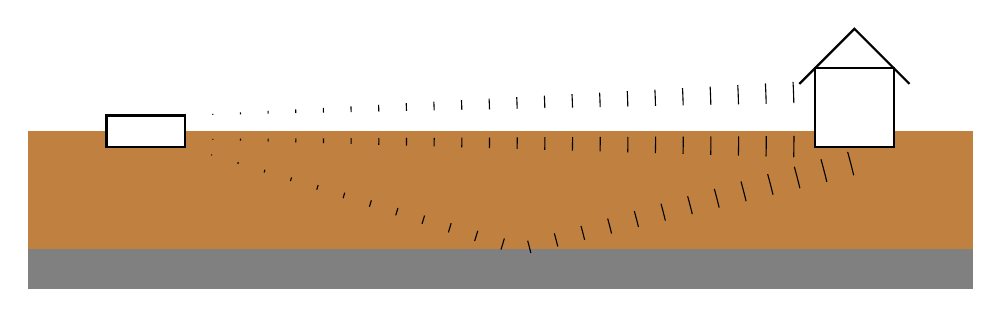
\begin{tikzpicture}
 \fill[color=brown] (-6,-1.5) rectangle (6, 0);
 \fill[color=gray] (-6,-2) rectangle (6,-1.5);
 \draw[thick, fill=white] (-5,-0.2)  rectangle (-4, 0.2);
 \draw[thick, fill=white] ( 4,-0.2)  rectangle ( 5, 0.8);
 \draw[thick] (3.8, 0.6) -- (4.5, 1.3) -- (5.2, 0.6);
 \draw[decorate,decoration={expanding waves, angle=1}] (-4, 0.2) -- (4, 0.5);
 \draw[decorate,decoration={expanding waves, angle=1}] (-4,-0.1) -- (4,-0.2);
 \draw[decorate,decoration={expanding waves, angle=1}] (-4,-0.2) -- (0.25,-1.5) -- (4.5,-0.4);
\end{tikzpicture}

\end{center}
\begin{description}[leftmargin=!,labelwidth=1mm]
\item[Quellen] Verkehr, Bauarbeiten, Maschinen, Naturereignisse
\item[Übertragungsweg] Boden (Dämpfung, Reflexion, Transmission) und Luft (hier nicht betrachtet) 
\item[Empfänger] Gebäude(teile), Lebewesen, Geräte
\end{description}
\end{frame}


\begin{frame}
\frametitle{Erschütterungsemission {\normalsize durch Verkehr}}
Logarithmische Darstellung der Partikelgeschwindigkeit \cite{studer2008bodendynamik}
\begin{equation*}
 L_v=\mathrm{dB}(v)=20\log\left(\frac{v}{v_\mathrm{ref}}\right)
\end{equation*}
bezogen auf den Referenzwert $v_\mathrm{ref}=\SI{1e-6}{\milli\metre\per\second}$ (ISO 1683).
Damit folgende Übertragungsverluste und -verstärkungen
\begin{equation*}
L_\mathrm{immision}=L_\mathrm{emision}
\underbrace{-\Delta L_{v,\mathrm{geom}}-\Delta L_{v,\mathrm{mat}}- \Delta L_{v,\mathrm{refl}}}_{\text{Verluste im Übertragungsmedium}}
\underbrace{-\Delta L_{v,\mathrm{koppl}}-\Delta L_{v,\mathrm{empf}}}_{\text{Verluste/Verst. am Empfänger}}
\end{equation*}
TODO fig 5.6 \cite{studer2008bodendynamik}
\end{frame}


\begin{frame}
\frametitle{Erschütterungsemission {\normalsize durch Bauarbeiten}}
Speziell für Spreng- und Rammerschütterungen \cite{studer2008bodendynamik} ist die Messung an der Quelle schwierig, deswegen wird die eingebrachte Energie als Kenngröße benutzt
\begin{equation*}
 v=cW^\alpha r^\beta.
\end{equation*}
TODO Details

Maschinen sind Punktequellen und werden nach der gleichen Formel geschätzt \cite{studer2008bodendynamik}.
\end{frame}


\begin{frame}
\frametitle{Erschütterungseinwirkung}

TODO fig 5.11 \cite{studer2008bodendynamik} % Belästigung (subjektiv) vor Schädigung
TODO fig 5.12 \cite{studer2008bodendynamik} % Messort entscheidend

\end{frame}

\begin{frame}
\frametitle{Erschütterungseinwirkung {\normalsize auf Bauwerke}}
Deutschland DIN 4150-3 (1999) Erschütterungen im Bauwesen, Einwirkungen
auf bauliche Anlagen.
 VDI 2716 (2001 mit Berichtigungen 2003) Luft- und Körperschall
bei Schienenbahnen des öffentlichen Personennahverkehrs

Kennwert Partikelgeschwindigkeitsvektor

Schweiz
Häufigkeitsklassen: gelegentlich, häufig, permanent
Empfindlichkeitsklassen: sehr wenig/wenig/normal/erhöht empfindlich 
Richtwerte
\cite{studer2008bodendynamik}

\end{frame}


\begin{frame}
\frametitle{Erschütterungseinwirkung {\normalsize auf Menschen}}
Kriterien \cite{studer2008bodendynamik}
Deutschland  DIN 4150-2 (1999) Erschütterungen im Bauwesen, Einwirkungen
auf Menschen in Gebäuden. DIN Deutsches Institut für Normung
VDI 2057 (2002) Einwirkung mechanischer Schwingungen auf den
Menschen, Blatt 1, 2 und 3, VDI Verein Deutscher Ingenieure

Schwingung und (primär, sekundär) Schall (unterschiedlich gewichtet in Normen)
TODO fig 5.16 \cite{studer2008bodendynamik}
\end{frame}


\begin{frame}
\frametitle{Erschütterungseinwirkung{\normalsize auf Geräte}}
ISO 8569:1996 Mechanical vibration and shock – Measurement and evaluation of
shock and vibration effects on sensitive equipment in buildings
\cite{studer2008bodendynamik}

\end{frame}


\begin{frame}
\frametitle{Erschütterungsreduktion}
\cite{studer2008bodendynamik}

Quelle: optimiertes Sprengschema, Maschinenfundamente, Unterschottermatten, Zusatzmassen/fundament

Übertragungsmedium: Schlitze TODO fig 6.19

Empfänger: Auflagerung/Fundament, Schwingungstilger (2dof)
\end{frame}


\begin{frame}
\frametitle{Beispiel}
4.3.3 \cite{haupt1986bodendynamik}
\end{frame}




\subsection{Erdbebensicheres Bauen}


\begin{frame}
\frametitle{Erdbeben}
123
\end{frame}




%%%%%%%%%%%%%%%%%%%%%%%%%%%%%%%%%%%%%%%%%%%%%%%%

\section*{Literaturverzeichnis}

\begin{frame}[allowframebreaks]{}
	\printbibliography
\end{frame}
\end{document}
